\documentclass{article}
\usepackage{tikz}
\usepackage{pifont}
\usepackage[fontsize=16pt]{fontsize}

\title{Real Numbers}
\author{Applied Scholastics Ferndale}\\
\date{}

\begin{document}

\maketitle
\newpage

\large
\section*{Real numbers}

\vspace{16pt}
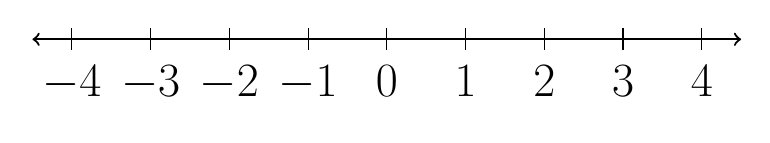
\begin{tikzpicture}
	\draw [<->,thick](-4.5,0) -- (4.5,0);
	\foreach \x in {-4,...,4}
	\draw (\x,4pt) -- +(0,-8pt) node [below] {$\x$};
\end{tikzpicture}\\

Integers can be represented as specially-marked points evenly spaced on a line, but that only includes whole numbers. Real numbers are every possible point on the line including the integers. That includes all fractions, decimal fractions, and all roots of numbers.\\

\vspace{16pt}
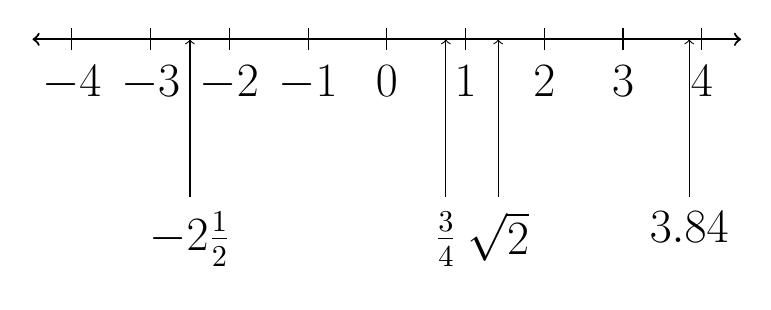
\begin{tikzpicture}
	\draw [<->,thick](-4.5,0) -- (4.5,0);
	\foreach \x in {-4,...,4}
	\draw (\x,4pt) -- +(0,-8pt) node [below] {$\x$};
	\draw [<-] (-2.5,0) -- (-2.5,-2) node [below] {$-2\frac{1}{2}$};
	\draw [<-] (1.4142,0) -- (1.4142,-2) node [below] {$\sqrt{2}$};
	\draw [<-] (0.75,0) -- (0.75,-2) node [below] {$\frac{3}{4}$};
	\draw [<-] (3.84,0) -- (3.84,-2) node [below] {$3.84$};
\end{tikzpicture}\\

They are called real numbers because they represent amounts in the real world.\\

\newpage

\subsection*{Rational Numbers}

A ratio is an amount of one thing compared to an amount of some other thing. A "3 to 4" ratio means that there are 3 of something for every 4 of something else. A ratio can also be expressed as a fraction. For a 3 to 4 ratio, $\frac{3}{4}$ of the total amount must be something and $\frac{1}{4}$ of it must make up the rest.\\

If a number can be expressed exactly as a ratio of two numbers, such as $\frac{3}{4}$ or $\frac{-6}{5}$, then it is called a rational number.\\

Integers and whole numbers are rational numbers as well because they can all be expressed as a ratio of themselves to one, such as $3=\frac{3}{1}$ or $-27=\frac{-27}{1}$.\\

\subsection*{Irrational Numbers}

Real numbers that can't be written as a ratio of two other numbers are called irrational numbers.\\

Irrational numbers can be precisely defined, such as $\pi = \frac{circumference}{diameter}$ or $\sqrt{2}$, but they cannot be written as a ratio or fraction, and the digits as a decimal fraction would go on forever.\\

\subsubsection*{Terminating and Non-Terminating\\Decimal Fractions}

The digits in a decimal fraction will either terminate at some point, such as 3.752, or a digits will repeat itself endlessly, such as in $\frac{1}{9}=0.1111\dots$, or a sequence of numbers will start to repeat endlessly, such as in $\frac{22}{7}=3.142857142857\dots$, or digits will go on forever without repeating, as in the value of $\pi = 3.14159\dots$.\\

An endlessly repeating digit of a decimal fraction is marked by putting a dot above that digit, such as $\frac{1}{3}=0.333\ldots=0.\dot{3}.$\\

An endlessly repeating series of digits such as in $\frac{22}{7}=3.142857142857142857\dots$ is written as $3.\overline{142857}$ with a line drawn over the repeating part of the decimal.\\

Every rational number can be written as either a repeating or terminating decimal fraction. All repeating decimal fractions can be converted to exact fractions or ratios.\\

Decimal fractions that do not repeat or terminate are irrational numbers.\\

\newpage
\
\newpage
\
\newpage
\

\begin{center}
\linespread{2}\large

Enquiries

\textbf{Applied Scholastics Ferndale}

Principal: Paula McLennan

mobile phone: 0431 683 306

email address: apsferndale@gmail.com

website: apsferndale.webs.com
\end{center}

\end{document}
